\documentclass[10pt,xcolor=pst,aspectratio=169]{beamer}

\usepackage{etex}

%\usetheme{Boadilla}
%\usecolortheme{wolverine}
\usecolortheme{dolphin}
%\setbeamercovered{transparent}
%\setbeamercolor{block body}{bg=yellow}

\addtobeamertemplate{navigation symbols}{}{%
	\usebeamerfont{footline}%
	\usebeamercolor[fg]{footline}%
	\hspace{1em}%
	\insertframenumber/\inserttotalframenumber
}

\usepackage[utf8]{inputenc}
\usepackage[english,russian]{babel}
\usepackage[OT1]{fontenc}
\usepackage{amsmath, bm}
\usepackage{amsfonts}
\usepackage{amssymb}
\usepackage{graphicx}
\usepackage{wrapfig}
\usepackage[3D]{movie15}
\usepackage{animate}
\usepackage{ragged2e}
\usepackage{listings}
\usepackage{color}
\usepackage{pst-all}

\usepackage{tikz}
\usetikzlibrary{
	mindmap,
	arrows, % стрелки
	shapes.misc, % фигуры
	chains, % цепочки
	positioning, % позиционирование элементов
	scopes, % создание дополнительных веток
	shadows % тени
}

\graphicspath{{pic/}}

\author{\textbf{Губкин А.С.}}

\title[Численные методы в физике]{Численные методы в физике}

\logo{
\includegraphics[width=0.1\linewidth]{LOGO_2.EPS}}

\institute[ТюмФ ИТПМ СО РАН]{Тюменский филиал Института теоретической и прикладной механики\\ им. С. А. Христиановича СО РАН, г. Тюмень}

%\date{6 октября 2015 г.}

\begin{document}

\lstset{ %
	language=[ANSI]C++,                 % выбор языка для подсветки (здесь это С++)
	keywordstyle=\color{blue},
	commentstyle=\color{gray},
	basicstyle=\scriptsize,
%basicstyle=\small\sffamily, % размер и начертание шрифта для подсветки кода
	numbers=left,               % где поставить нумерацию строк (слева\справа)
	numberstyle=\tiny,           % размер шрифта для номеров строк
%stepnumber=1,                   % размер шага между двумя номерами строк
	numbersep=4pt,                % как далеко отстоят номера строк от подсвечиваемого кода
%backgroundcolor=\color{white}, % цвет фона подсветки - используем \usepackage{color}
	showspaces=false,            % показывать или нет пробелы специальными отступами
	showstringspaces=false,      % показывать или нет пробелы в строках
	showtabs=false,             % показывать или нет табуляцию в строках
	frame=single,              % рисовать рамку вокруг кода
%tabsize=2,                 % размер табуляции по умолчанию равен 2 пробелам
	captionpos=t,              % позиция заголовка вверху [t] или внизу [b] 
	breaklines=true,           % автоматически переносить строки (да\нет)
	breakatwhitespace=true, % переносить строки только если есть пробел
	escapeinside={\%*}{*)}   % если нужно добавить комментарии в коде
}

%SLIDE #1
\begin{frame}

	\transdissolve[duration=0.1]
	\titlepage

\end{frame}

%SLIDE #?
\begin{frame}{Введение}

	\transdissolve[duration=0.1]
	\justifying
	\large

	Рассмотрим одномерный гиперболический закон сохранения:
	\[
		u_{t} + f(u)_{x} = 0.
	\]
	Будем рассматривать два потока $f(u)$: $\frac{u^{2}}{2}$, $\frac{u^{2}}{u^{2} + \frac{1}{4}(1 - u^{2})^2}$ - поток уравнения Бюргерса и поток уравнения Баклея - Леверетта соответственно.

\end{frame}

%SLIDE #?
\begin{frame}{Введение}

	\transdissolve[duration=0.1]
	\justifying
	\large

	\begin{center}
		\tikzstyle{root concept}+=[concept color=blue!80,minimum size=3.5cm]
		\tikz[mindmap]
			\node [concept] {Основные подходы}
				child[concept color=yellow, grow=130, minimum size=2.5cm]
				{
					node[concept](root1) at (0,0) {Методы выделения разрывов}
					node[annotation,left] at (root1.south)
					{
						\begin{itemize}
							\item[$\oplus$] очень точно определяются положение и величина разрыва;
							\item[$\ominus$] сложное программирование/реализация;
							\item[$\ominus$] в задачах со сложной динамикой возникают проблемы с сеткой.
						\end{itemize}
					}
				}
				child[concept color=green, grow=50, minimum size=2.5cm]
				{
					node[concept](root2) at (0,0) {Схемы сквозного счета}
					node[annotation,right] at (root2.south)
					{
						\begin{itemize}
							\item[$\oplus$] относитльно простая реализация;
							\item[$\oplus$] применимы для широкого класса задач;
							\item[$\ominus$] численная диссипация приводит к "размазыванию" разрывов;
							\item[$\ominus$] численная дисперсия приводит к появленю осцилляций вблизи разрывов.
						\end{itemize}
					}
				};
	\end{center}

\end{frame}

%SLIDE #?

\begin{frame}{Метод контрольного объема/МКО (Finite Volume Method/FVM)}

	\transdissolve[duration=0.1]
	\justifying
	\large

	\[
		\frac{\partial \vec{s}}{\partial t} + \vec{\nabla} \cdot f (\vec{s}) = 0.
	\]
	
	\[
		\begin{split}
			&\frac{\partial \vec{s}}{\partial t} + \vec{\nabla} \cdot f (\vec{s}) = 0 \Rightarrow
			\int_{v_{i}} \frac{\partial \vec{s}}{\partial t} d v + \int_{v_{i}} \vec{\nabla} \cdot f (\vec{s}) d v = 0 \Rightarrow \\
			&v_{i} \frac{d \tilde{\vec{s}}_{i}}{d t} + \int_{\sigma_{i}} f (\vec{s}) \cdot \vec{n} d \sigma = 0 \Rightarrow
			\frac{d \tilde{\vec{s}}_{i}}{d t} + \frac{1}{v_{i}} \sum_{\sigma_{i}} \tilde{f} (\tilde{\vec{s}}) \cdot \vec{\sigma_{i}} = 0.
		\end{split}
	\]

\end{frame}

\begin{frame}{Схема к методу контрольного объема}

	\transdissolve[duration=0.1]
	\justifying
	\large

	\[
		\frac{d \tilde{\vec{s}}_{i}}{d t} + \frac{1}{v_{i}} \sum_{\sigma_{i}} \tilde{f} (\tilde{\vec{s}}) \cdot \vec{\sigma_{i}} = 0.
	\]

	\begin{figure}
		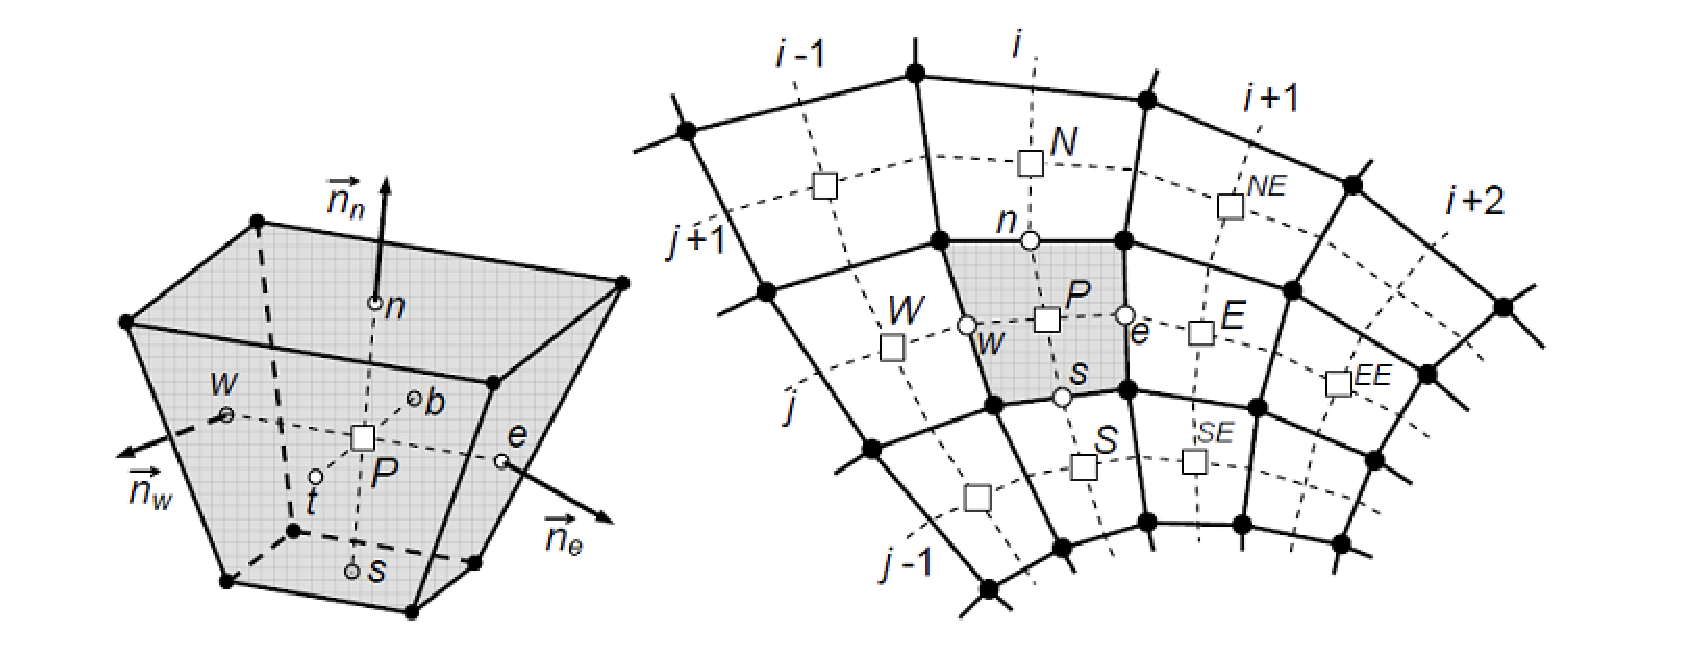
\includegraphics[width=0.8\linewidth]{FVM_scheme.eps}
	\end{figure}

\end{frame}

\begin{frame}{МКО в случае одной пространственной переменной}

	\transdissolve[duration=0.1]
	\justifying
	\large

	В случае одной пространственной переменной предыдущее уравнение примет вид:

	\[
		\frac{d u_{i}}{d t} + \frac{1}{\Delta x_{i}} \left( f_{i + \frac{1}{2}} - f_{i - \frac{1}{2}} \right) = 0,
	\]

	где $\Delta x_{i} = x_{i + \frac{1}{2}} - x_{i - \frac{1}{2}}$, $f_{i + \frac{1}{2}} = f \left( u^{n}_{i - \xi} \ldots u^{n}_{i + \eta} \right)$ - численный поток, $\xi$ и $\eta$ - определяют шаблон разностной схемы.

\end{frame}

%SLIDE #?
\begin{frame}{Шаблон разностной схемы}

	\transdissolve[duration=0.1]
	\justifying
	\large

	\begin{block}{Определение}
		\justifying
		\textbf{Шаблон} -- это мнемоническая диаграмма, которая указывает способ образования разностной схемы, показывая точки разностной сетки, участвующие в аппроксимации.
	\end{block}
 
\end{frame}

%SLIDE #?
\begin{frame}{Пример шаблона}

	\transdissolve[duration=0.1]
	\justifying
	\large

	\[
		u_{t} + a u_{x} = 0 \Rightarrow
			\begin{cases}
				&\frac{u^{n + 1}_{i} - u^{n}_{i}}{\Delta t} + a \frac{u^{n}_{i} - u^{n}_{i - 1}}{\Delta x} = 0, \quad a > 0, \\
				&\frac{u^{n + 1}_{i} - u^{n}_{i}}{\Delta t} + a \frac{u^{n}_{i + 1} - u^{n}_{i - 1}}{\Delta x} = 0, \quad a > 0, \\
				&\frac{u^{n + 1}_{i} - u^{n}_{i}}{\Delta t} + a \frac{u^{n}_{i + 1} - u^{n}_{i}}{\Delta x} = 0, \quad a > 0.
			\end{cases}
	\]

	\begin{center}
		\psset{xunit=1cm,yunit=1cm,algebraic=true}
		\begin{pspicture}(0,0)(8,3)
			\psgrid[griddots=20, gridwidth=0pt, gridcolor=gray, gridlabels=0pt, subgriddiv=1, subgriddots=20, subgridcolor=gray](0,0)(0,0)(8,3)
			\psaxes[Dx=1, Dy=1, subticks=1, labelFontSize=\scriptscriptstyle]{-}(0,0)(0,0)(8,3)[$x_{i}$,0][$t_{n}$,90]

			\psline[linewidth=2pt, linecolor=red]{o-o}(1,1)(2,1)
			\psline[linewidth=2pt, linecolor=red]{o-o}(2,1)(2,2)
			\uput[-90](1,1){\scriptsize $(i - 1, n)$}
			\uput[-90](2,1){\scriptsize $(i, n)$}
			\uput[90](2,2){\scriptsize $(i, n + 1)$}

			\psline[linewidth=2pt, linecolor=red]{o-o}(3,1)(4,1)
			\psline[linewidth=2pt, linecolor=red]{o-o}(4,1)(5,1)
			\psline[linewidth=2pt, linecolor=red]{o-o}(4,1)(4,2)
			\uput[-90](3,1){\scriptsize $(i - 1, n)$}
			\uput[-90](4,1){\scriptsize $(i, n)$}
			\uput[-90](5,1){\scriptsize $(i + 1, n)$}
			\uput[90](4,2){\scriptsize $(i, n + 1)$}

			\psline[linewidth=2pt, linecolor=red]{o-o}(6,1)(7,1)
			\psline[linewidth=2pt, linecolor=red]{o-o}(6,1)(6,2)
			\uput[-90](6,1){\scriptsize $(i, n)$}
			\uput[-90](7,1){\scriptsize $(i + 1, n)$}
			\uput[90](6,2){\scriptsize $(i, n + 1)$}

		\end{pspicture}
	\end{center}
 
\end{frame}

%SLIDE #?
\begin{frame}{Шаблон в общем одномерном случае}

	\transdissolve[duration=0.1]
	\justifying
	\large

	\begin{center}
		\psset{xunit=1cm,yunit=1cm,algebraic=true}
		\begin{pspicture}(0,0)(8,3)
			\psgrid[griddots=20, gridwidth=0pt, gridcolor=gray, gridlabels=0pt, subgriddiv=1, subgriddots=20, subgridcolor=gray](0,0)(0,0)(8,3)
			\psaxes[Dx=1, Dy=1, subticks=1, labelFontSize=\scriptscriptstyle]{-}(0,0)(0,0)(8,3)[$x_{i}$,0][$t_{n}$,90]

			\psline[linewidth=2pt, linecolor=red]{o-o}(1,1)(2,1)
			\psline[linewidth=2pt, linecolor=red]{o-o}(2,1)(3,1)
			\psline[linewidth=2pt, linecolor=red]{o-o}(3,1)(4,1)
			\psline[linewidth=2pt, linecolor=red]{o-o}(4,1)(5,1)
			\psline[linewidth=2pt, linecolor=red]{o-o}(5,1)(6,1)
			\psline[linewidth=2pt, linecolor=red]{o-o}(6,1)(7,1)
			\psline[linewidth=2pt, linecolor=red]{o-o}(4,1)(4,2)
			\uput[-90](1,1){\scriptsize $(i - \xi, n)$}
			\uput[-90](2,1){\scriptsize $\ldots$}
			\uput[-90](3,1){\scriptsize $(i - 1, n)$}
			\uput[-90](4,1){\scriptsize $(i, n)$}
			\uput[-90](5,1){\scriptsize $(i + 1, n)$}
			\uput[-90](6,1){\scriptsize $\ldots$}
			\uput[-90](7,1){\scriptsize $(i + \eta, n)$}
			\uput[90](4,2){\scriptsize $i, n + 1$}

		\end{pspicture}
	\end{center}
 
\end{frame}

%SLIDE #?
\begin{frame}{Дискретизация по пространству}

	\transdissolve[duration=0.1]
	\justifying
	\normalsize

	Различные версии метода контрольного объема отличаются способом вычисления потоков:

	\begin{center}
		\tikzstyle{root concept}+=[concept color=blue!80,minimum size=3cm]
		\tikz[mindmap]
			\node [concept] {Методы расчета потоков}
				child[concept color=yellow, grow=140, minimum size=2cm]
				{
					node[concept](root1) at (0,-1) {\textbf{Flux method}\\$f = f(u)$}
				}
				child[concept color=green, grow=190, minimum size=3cm]
				{
					node[concept](root2) at (0,0) {\textbf{Flux Vector Splitting}\\$f = f^{+}(u) + f^{-}(u)$}
				}
				child[concept color=red, grow=0, minimum size=4cm]
				{
					node[concept](root2) at (0.5,0) {\textbf{Reconstruction - Evolution}\\$f = f \left( u^{+} + u^{-} \right)$}
				};
	\end{center}

\end{frame}

%SLIDE #?
\begin{frame}{Методы расчета потоков}

	\transdissolve[duration=0.1]
	\justifying
	\large

	Простейший способ вычисления потока как полусуммы соответствующих величин на гранях контрольного объема:

	\[
		f_{i + \frac{1}{2}} = \frac{1}{2} \left( f_{i + 1} + f_{i} \right),
	\]

	приводит к нейстойчивости разностной схемы.

\end{frame}

%SLIDE #?
\begin{frame}{Монотонность схемы}

	\transdissolve[duration=0.1]
	\justifying
	\large

	Условие монотонности схемы для уравнения

	\[
		u_{t} + f(u)_{x} = 0
	\]
	
	заключается в том, что для двух заданных начальных данных, таких, что одно везде больше другого: $u(x, 0) \geq w(x, 0)$, в последующие моменты времени это свойство сохраняется: $u(x, t) \geq w(x, t)$.

\end{frame}

%SLIDE #?
\begin{frame}{Монотонность схемы}

	\transdissolve[duration=0.1]
	\justifying
	\large

	Для конечно-разностной схемы

	\[
		u_{i}^{n + 1} = H \left( u_{i - m}^{n}, \cdots, u_{i}^{n}, \cdots, u_{i + m}^{n} \right)
	\]

	условие монотонности имеет вид

	\[
		\frac{\partial H}{\partial u_{i + j}^{n}} \geq 0, \: j \in [-m, m].
	\]

\end{frame}

%SLIDE #?
\begin{frame}{Теорема Годунова}

	\transdissolve[duration=0.1]
	\justifying
	\large

	\newtheorem{Th}{Теорема}
	\begin{Th}[Годунов С.К.]
		\justifying
		Для того чтобы разностная схема вида

		\[
			u_{i}^{n + 1} = \sum_{j} a_{j} u_{j}^{n}
		\]
		
		переводила все монотонные функции в монотонные с тем же направлением роста, необходимо и достаточно, чтобы все коэффициенты $a_{j}$ были неотрицательными.
	\end{Th}

\end{frame}

%SLIDE #?
\begin{frame}{Монотонность схемы}

	\transdissolve[duration=0.1]
	\justifying
	\large

	Из условий

	\[
		\sum_{j} a_{j} = 1, \: a_{j} \geq 0
	\]

	вытекает, что

	\[
		\max_{i} \left| u_{i}^{n + 1} \right| \leq \left| a_{j} \right| \max_{j} \left| u_{j}^{n} \right|
	\]

	так как $\left| a_{j} \right| \leq 1$, то получаем условие устойчивости монотонных схем

	\[
		\sum_{i} \left| u_{i}^{n + 1} \right| \leq \sum_{j} \left| u_{j}^{n} \right|.
	\]

\end{frame}

%SLIDE #?
\begin{frame}{Следствие}

	\transdissolve[duration=0.1]
	\justifying
	\large

	\newtheorem{Th2}{Следствие}
	\begin{Th2}[Годунов С.К.]
		\justifying
		Среди линейных разностных схем второго порядка точности для уравнения $u_{t} + u_{x}$ \textbf{нет схем}, удовлетворяющих условию монотонности.
	\end{Th2}

\end{frame}

%SLIDE #?
\begin{frame}{Пример}

	\transdissolve[duration=0.1]
	\justifying
	\large

	Рассмотрим семейство трехточечных явных схем для линейного уравнения переноса:

	\[
		u_{i}^{n + 1} = a u_{i - 1}^{n} + b u_{i}^{n} + c u_{i + 1}^{n}.
	\]

	Это соотношение можно переписать в форме, гарантирующем консервативность:

	\[
		\begin{split}
			&u_{i}^{n + 1} = u_{i}^{n} - \frac{1}{2} \left[ \varepsilon_{i + 1/2} (u_{i + 1}^{n} + u_{i}^{n}) - \varepsilon_{i - 1/2} (u_{i}^{n} + u_{i - 1}^{n})\right] + \\
			& + \left[ \nu_{i + 1/2} (u_{i + 1}^{n} + u_{i}^{n}) - \nu_{i - 1/2} (u_{i}^{n} + u_{i - 1}^{n})\right].
		\end{split}
	\]

\end{frame}

%SLIDE #?
\begin{frame}{Пример}

	\transdissolve[duration=0.1]
	\justifying
	\large

	Тогда коэффициенты будут:

	\[
		\begin{split}
			&a = \nu_{i - 1/2} + \frac{1}{2} \varepsilon_{i - 1/2}, \\
			&b = 1 - \frac{1}{2} \varepsilon_{i + 1/2} + \frac{1}{2} \varepsilon_{i - 1/2} - \nu_{i + 1/2} - \nu_{i - 1/2},\\
			&c = \nu_{i + 1/2} - \frac{1}{2} \varepsilon_{i + 1/2}.
		\end{split}
	\]

\end{frame}

%SLIDE #?
\begin{frame}{Метод Лакса - Фридрихса (Lax - Friedrichs)}

	\transdissolve[duration=0.1]
	\justifying
	\large

	Одним из первых разностных методов предназначеных для дискретизации гиперболического закона сохранения (уравнения Эйлера) был метод Лакса - Фридрихса (1954):
	
	\[
		f_{i + \frac{1}{2}} = \frac{1}{2} \left( f_{i + 1} + f_{i} \right) - 
		\frac{\Delta x}{2 \Delta t} \left( u_{i + 1} - u_{i} \right),
	\]

	\[
		f_{i - \frac{1}{2}} = \frac{1}{2} \left( f_{i} + f_{i - 1} \right) - 
		\frac{\Delta x}{2 \Delta t} \left( u_{i} - u_{i - 1} \right).
	\]

	Метод Лакса - Фридрихса оказался слишком диффузонным и широкого распространения не получил.

\end{frame}

%SLIDE #?
\begin{frame}{Начальное условие}

	\transdissolve[duration=0.1]
	\justifying
	\large

	\[
		u(x,0) =
		\begin{cases}
			&\frac{3}{4} \qquad x = 0\\
			&0 \qquad x \geq 0
		\end{cases}
	\]

	\begin{center}
		\psset{xunit=4cm,yunit=4cm,algebraic=true}
		\begin{pspicture}(0,0)(2,1)
			\psgrid[griddots=20, gridwidth=0pt, gridcolor=gray, gridlabels=0pt, subgriddiv=5, subgriddots=20, subgridcolor=gray](0,0)(0,0)(2,1)
			\psaxes[Dx=0.2, Dy=0.2, subticks=2, labelFontSize=\scriptscriptstyle]{-}(0,0)(0,0)(2,1)[$x$,0][$u$,90]
			\psline[linewidth=2pt, linecolor=blue]{*}(0,0.75)(0,0.75)
			\uput[0](0,0.75){$u = \frac{3}{4}$}
			\psplot[linewidth=2pt, linecolor=blue, yMaxValue=1, yMinValue=0]{0}{2} {0}
		\end{pspicture}
	\end{center}

\end{frame}

%SLIDE #?
\begin{frame}{Метод Лакса - Фридрихса}

	\transdissolve[duration=0.1]
	\justifying
	\large

	%ANIMATION #
%    \begin{figure}[h]
%	    \center{\animategraphics[autoplay, controls=true, width=0.5\linewidth]{50}{tests/eps/BEqnLaxFriedrichs/BEqnLaxFriedrichs.}{0}{299}}
%    \end{figure}

	\vspace{-1ex}

	\begin{minipage}{0.49\textwidth}
		\begin{center}
			уравнение Бюргерса
		\end{center}
	\end{minipage}
	\hfill
	\begin{minipage}{0.49\textwidth}
		\begin{center}
			уравнение Баклея - Леверетта
		\end{center}
	\end{minipage}

	\begin{minipage}{0.49\textwidth}
		\begin{center}
			\movie[label=cells,width=7cm,height=6cm,loop,poster,showcontrols]{\includegraphics[width=7cm,height=6cm]{tests/eps/BEqnLaxFriedrichs/BEqnLaxFriedrichs.0.eps}}{tests/png/BEqnLaxFriedrichs.mp4}
		\end{center}
	\end{minipage}
	\hfill
	\begin{minipage}{0.49\textwidth}
		\begin{center}
			\movie[label=cells,width=7cm,height=6cm,loop,poster,showcontrols]{\includegraphics[width=7cm,height=6cm]{tests/eps/BLEqnLaxFriedrichs/BLEqnLaxFriedrichs.0.eps}}{tests/png/BLEqnLaxFriedrichs.mp4}
		\end{center}
	\end{minipage}

\end{frame}

%%SLIDE #?
%\begin{frame}{Численное решение уравнения Баклея - Леверетта (метод Лакса - Фридрихса)}
%
%	\transdissolve[duration=0.1]
%	\justifying
%	\large
%
%	%ANIMATION #
%    \begin{figure}[h]
%	    \center{\animategraphics[autoplay, controls=true, width=0.5\linewidth]{50}{tests/eps/BLEqnLaxFriedrichs/BLEqnLaxFriedrichs.}{0}{299}}
%    \end{figure}
%
%\end{frame}

%SLIDE #?
\begin{frame}{Метод Лакса - Вендрофа (Lax - Wendroff)}

	\transdissolve[duration=0.1]
	\justifying
	\large

	Метод Лакса - Вендрофа (1960) имеет второй порядок точности по пространству. Поток расчитывается следующим образом:

	\[
		f_{i + \frac{1}{2}} = \frac{1}{2} \left( f_{i + 1} + f_{i} \right) - 
		\frac{1}{2} a_{i + \frac{1}{2}}^{2} \frac{\Delta t}{\Delta x} \left( u_{i + 1} - u_{i} \right),
	\]

	где $a_{i + 1/2}$ расчитывается как

	\[
		a_{i + \frac{1}{2}} =
		\begin{cases}
			&\frac{f_{i + 1} - f_{i}}{u_{i + 1} - u_{i}}, \: u_{i + 1} \neq u_{i} \\
			&f'(u_{i}), \: u_{i + 1} = u_{i}.
		\end{cases}
	\]
	
	Метод Лакса - Вендрофа приводит к нефизическим осцилляциям решения.

\end{frame}

%%SLIDE #?
%\begin{frame}{Численное решение уравнения Бюргерса (метод Лакса - Вендрофа)}
%
%	\transdissolve[duration=0.1]
%	\justifying
%	\large
%
%	%ANIMATION #
%    \begin{figure}[h]
%	    \center{\animategraphics[autoplay, controls=true, width=0.5\linewidth]{50}{tests/eps/BEqnLaxWendroffMuA0/BEqnLaxWendroff.}{0}{199}}
%    \end{figure}
%
%\end{frame}
%
%%SLIDE #?
%\begin{frame}{Численное решение уравнения Баклея - Леверетта (метод Лакса - Вендрофа)}
%
%	\transdissolve[duration=0.1]
%	\justifying
%	\large
%
%	%ANIMATION #
%    \begin{figure}[h]
%	    \center{\animategraphics[autoplay, controls=true, width=0.5\linewidth]{50}{tests/eps/BLEqnLaxWendroffMuA0/BLEqnLaxWendroff.}{0}{199}}
%    \end{figure}
%
%\end{frame}

%SLIDE #?
\begin{frame}{Метод Лакса - Вендрофа}

	\transdissolve[duration=0.1]
	\justifying
	\large

	\vspace{-1ex}

	\begin{minipage}{0.49\textwidth}
		\begin{center}
			уравнение Бюргерса
		\end{center}
	\end{minipage}
	\hfill
	\begin{minipage}{0.49\textwidth}
		\begin{center}
			уравнение Баклея - Леверетта
		\end{center}
	\end{minipage}

	\begin{minipage}{0.49\textwidth}
		\begin{center}
			\movie[label=cells,width=7cm,height=6cm,loop,poster,showcontrols]{\includegraphics[width=7cm,height=6cm]{tests/eps/BEqnLaxWendroffMuA0/BEqnLaxWendroff.0.eps}}{tests/png/BEqnLaxWendroffMuA0.mp4}
		\end{center}
	\end{minipage}
	\hfill
	\begin{minipage}{0.49\textwidth}
		\begin{center}
			\movie[label=cells,width=7cm,height=6cm,loop,poster,showcontrols]{\includegraphics[width=7cm,height=6cm]{tests/eps/BLEqnLaxWendroffMuA0/BLEqnLaxWendroff.0.eps}}{tests/png/BLEqnLaxWendroffMuA0.mp4}
		\end{center}
	\end{minipage}

\end{frame}

%SLIDE #?
\begin{frame}{Двухшаговый метод Лакса - Вендрофа}

	\transdissolve[duration=0.1]
	\justifying
	\large

	Чтобы избежать вычисления якобиана $\frac{f_{i + 1} - f_{i}}{u_{i + 1} - u_{i}}$, $\frac{f_{i} - f_{i - 1}}{u_{i} - u_{i - 1}}$ используется двухшаговая процедура, предложенная Рихтмаером (Richtmyer):
	
	Первый шаг:

	\[
		u^{n + \frac{1}{2}}_{i + \frac{1}{2}} = \frac{1}{2}(u^{n}_{i + 1} + u^{n}_{i}) - \frac{\Delta t}{2\,\Delta x} \left( f(u^{n}_{i + 1}) - f(u^{n}_{i}) \right),
	\]

	\[
		u^{n + \frac{1}{2}}_{i - \frac{1}{2}} = \frac{1}{2}(u^{n}_{i} + u^{n}_{i - 1}) - \frac{\Delta t}{2\,\Delta x} \left( f(u^{n}_{i}) - f(u^{n}_{i - 1}) \right).
	\]

	Второй шаг:

	\[
		u^{n+1}_{i} = u^{n}_{i} - \frac{\Delta t}{\Delta x} \left( f(u^{n + \frac{1}{2}}_{i + \frac{1}{2}}) - f(u^{n + \frac{1}{2}}_{i - \frac{1}{2}}) \right).
	\]

\end{frame}

%SLIDE #?
\begin{frame}{Искусственная вязкость}

	\transdissolve[duration=0.1]
	\justifying
	\large

	Введение искусственной вязкости приводит к затуханию высокочастотных компонентов решения в процессе вычислений, что можно использовать для подавления нефизических осцилляций разностного решения. Включение вязкости можно осуществить с помощью специальных членов.

\end{frame}

%SLIDE #?
\begin{frame}{Метод искусственной вязкости для метода Лакса - Вендрофа}

	\transdissolve[duration=0.1]
	\justifying
	\large

	\[
		\begin{split}
			&u^{n+1}_{i} = u^{n}_{i} - \frac{\Delta t}{\Delta x} \left( f(u^{n + \frac{1}{2}}_{i + \frac{1}{2}}) - f(u^{n + \frac{1}{2}}_{i - \frac{1}{2}}) \right) + \\
			&+ \mu_{a} \Delta t \left( u^{n}_{i + 1} - 2 u^{n}_{i} + u^{n}_{i - 1} \right).
		\end{split}
	\]

	Введение искусственной вязкости имеет смысл только для схем второго и выше порядков аппроксимации.\\

	Введение искусственной вязкости иногда бывает необходимым для получения устойчивого процесса вычислений.

\end{frame}

%%SLIDE #?
%\begin{frame}{Численное решение уравнения Бюргерса (метод Лакса - Вендрофа с искусственной вязкостью)}
%
%	\transdissolve[duration=0.1]
%	\justifying
%	\large
%
%	%ANIMATION #
%    \begin{figure}[h]
%	    \center{\animategraphics[autoplay, controls=true, width=0.5\linewidth]{50}{tests/eps/BEqnLaxWendroffMuA60/BEqnLaxWendroff.}{0}{299}}
%    \end{figure}
%
%\end{frame}
%
%%SLIDE #?
%\begin{frame}{Численное решение уравнения Баклея - Леверетта (метод Лакса - Вендрофа с искусственной вязкостью)}
%
%	\transdissolve[duration=0.1]
%	\justifying
%	\large
%
%	%ANIMATION #
%    \begin{figure}[h]
%	    \center{\animategraphics[autoplay, controls=true, width=0.5\linewidth]{50}{tests/eps/BLEqnLaxWendroffMuA60/BLEqnLaxWendroff.}{0}{299}}
%    \end{figure}
%
%\end{frame}

%SLIDE #?
\begin{frame}{Метод Лакса - Вендрофа с искусственной вязкостью}

	\transdissolve[duration=0.1]
	\justifying
	\large

	\vspace{-1ex}

	\begin{minipage}{0.49\textwidth}
		\begin{center}
			уравнение Бюргерса
		\end{center}
	\end{minipage}
	\hfill
	\begin{minipage}{0.49\textwidth}
		\begin{center}
			уравнение Баклея - Леверетта
		\end{center}
	\end{minipage}

	\begin{minipage}{0.49\textwidth}
		\begin{center}
			\movie[label=cells,width=7cm,height=6cm,loop,poster,showcontrols]{\includegraphics[width=7cm,height=6cm]{tests/eps/BEqnLaxWendroffMuA60/BEqnLaxWendroff.0.eps}}{tests/png/BEqnLaxWendroffMuA60.mp4}
		\end{center}
	\end{minipage}
	\hfill
	\begin{minipage}{0.49\textwidth}
		\begin{center}
			\movie[label=cells,width=7cm,height=6cm,loop,poster,showcontrols]{\includegraphics[width=7cm,height=6cm]{tests/eps/BLEqnLaxWendroffMuA60/BLEqnLaxWendroff.0.eps}}{tests/png/BLEqnLaxWendroffMuA60.mp4}
		\end{center}
	\end{minipage}

\end{frame}

%SLIDE #?
\begin{frame}{Upwind scheme}

	\transdissolve[duration=0.1]
	\justifying
	\large

	In computational physics, upwind schemes denote a class of numerical discretization methods for solving hyperbolic partial differential equations. Upwind schemes use an adaptive or solution - sensitive finite difference stencil to numerically simulate the direction of propagation of information in a flow field. The upwind schemes attempt to discretize hyperbolic partial differential equations by using differencing biased in the direction determined by the sign of the characteristic speeds.

	\begin{flushright}
		\textbf{Wikipedia}
	\end{flushright}

\end{frame}

%SLIDE #?
\begin{frame}{First - order upwind scheme}

	\transdissolve[duration=0.1]
	\justifying
	\large

	Численный поток расчитывается следующим образом:

	\[
		f_{i + \frac{1}{2}} =
			\begin{cases}
				&f_{i}, \quad a_{i + \frac{1}{2}} \geq 0 \\
				&f_{i + 1}, \quad a_{i + \frac{1}{2}} < 0
			\end{cases},
	\]

	\[
		f_{i - \frac{1}{2}} =
			\begin{cases}
				&f_{i - 1}, \quad a_{i - \frac{1}{2}} \geq 0 \\
				&f_{i}, \quad a_{i - \frac{1}{2}} < 0
			\end{cases},
	\]

\end{frame}

%SLIDE #?
\begin{frame}{First - order upwind scheme stencil}

	\transdissolve[duration=0.1]
	\justifying
	\large

	\begin{center}
		\psset{xunit=1.5cm,yunit=1.5cm,algebraic=true}
		\begin{pspicture}(0,0)(6,3)
			\psgrid[griddots=20, gridwidth=0pt, gridcolor=gray, gridlabels=0pt, subgriddiv=1, subgriddots=20, subgridcolor=gray](0,0)(0,0)(6,3)
			\psaxes[Dx=1, Dy=1, subticks=1, labelFontSize=\scriptscriptstyle]{-}(0,0)(0,0)(6,3)[$x_{i}$,0][$t_{n}$,90]

			\psline[linewidth=2pt, linecolor=red]{o-o}(1,1)(2,1)
			\psline[linewidth=2pt, linecolor=red]{o-o}(2,1)(2,2)
			\uput[-90](1,1){\scriptsize $(i - 1, n)$}
			\uput[-90](2,1){\scriptsize $(i, n)$}
			\uput[90](2,2){\scriptsize $(i, n + 1)$}
			\uput[0](1,1.5){\scriptsize $a_{i + \frac{1}{2}} \geq 0$}

			\psline[linewidth=2pt, linecolor=red]{o-o}(4,1)(5,1)
			\psline[linewidth=2pt, linecolor=red]{o-o}(4,1)(4,2)
			\uput[-90](4,1){\scriptsize $(i, n)$}
			\uput[-90](5,1){\scriptsize $(i + 1, n)$}
			\uput[90](4,2){\scriptsize $(i, n + 1)$}
			\uput[0](4,1.5){\scriptsize $a_{i + \frac{1}{2}} < 0$}

		\end{pspicture}
	\end{center}
 
\end{frame}

%%SLIDE #?
%\begin{frame}{Численное решение уравнения Бюргерса (First - order upwind scheme)}
%
%	\transdissolve[duration=0.1]
%	\justifying
%	\large
%
%	%ANIMATION #
%    \begin{figure}[h]
%	    \center{\animategraphics[autoplay, controls=true, width=0.5\linewidth]{50}{tests/eps/BEqnFirstOrderUpwind/BEqnFirstOrderUpwind.}{0}{299}}
%    \end{figure}
%
%\end{frame}
%
%%SLIDE #?
%\begin{frame}{Численное решение уравнения Баклея - Леверетта (First - order upwind scheme)}
%
%	\transdissolve[duration=0.1]
%	\justifying
%	\large
%
%	%ANIMATION #
%    \begin{figure}[h]
%	    \center{\animategraphics[autoplay, controls=true, width=0.5\linewidth]{50}{tests/eps/BLEqnFirstOrderUpwind/BLEqnFirstOrderUpwind.}{0}{299}}
%    \end{figure}
%
%\end{frame}

%SLIDE #?
\begin{frame}{First - order upwind scheme}

	\transdissolve[duration=0.1]
	\justifying
	\large

	\vspace{-1ex}

	\begin{minipage}{0.49\textwidth}
		\begin{center}
			уравнение Бюргерса
		\end{center}
	\end{minipage}
	\hfill
	\begin{minipage}{0.49\textwidth}
		\begin{center}
			уравнение Баклея - Леверетта
		\end{center}
	\end{minipage}

	\begin{minipage}{0.49\textwidth}
		\begin{center}
			\movie[label=cells,width=7cm,height=6cm,loop,poster,showcontrols]{\includegraphics[width=7cm,height=6cm]{tests/eps/BEqnFirstOrderUpwind/BEqnFirstOrderUpwind.0.eps}}{tests/png/BEqnFirstOrderUpwind.mp4}
		\end{center}
	\end{minipage}
	\hfill
	\begin{minipage}{0.49\textwidth}
		\begin{center}
			\movie[label=cells,width=7cm,height=6cm,loop,poster,showcontrols]{\includegraphics[width=7cm,height=6cm]{tests/eps/BLEqnFirstOrderUpwind/BLEqnFirstOrderUpwind.0.eps}}{tests/png/BLEqnFirstOrderUpwind.mp4}
		\end{center}
	\end{minipage}

\end{frame}

%SLIDE #?
\begin{frame}{Warming-Beam scheme}

	\transdissolve[duration=0.1]
	\justifying
	\normalsize

	Численный поток расчитывается следующим образом:

	\[
		\begin{split}
			&f_{i + \frac{1}{2}} = \frac{1}{4} \left( - f_{i + 2} + 3 f_{i + 1} + 3 f_{i} - f_{i - 1} \right) - a_{i + \frac{1}{2}}^{2} \frac{\triangle x}{4 \triangle t} \left( u_{i + 2} - u_{i + 1} + u_{i} - u_{i - 1} \right) \\
			&- \frac{s_{i + \frac{1}{2}}}{4} \left( - f_{i + 2} + 3 f_{i + 1} - 3 f_{i} + f_{i - 1} \right) - s_{i + \frac{1}{2}} a_{i + \frac{1}{2}}^{2} \frac{\triangle x}{4 \triangle t} \left( u_{i + 2} - u_{i + 1} - u_{i} + u_{i - 1} \right).
		\end{split}
	\]

	\[
		s_{i + \frac{1}{2}} = \frac{a_{i + \frac{1}{2}}}{\left| a_{i + \frac{1}{2}} \right|}.
	\]

\end{frame}

%SLIDE #?
\begin{frame}{Warming-Beam scheme stencil}

	\transdissolve[duration=0.1]
	\justifying
	\large

	\begin{center}
		\psset{xunit=1.5cm,yunit=1.5cm,algebraic=true}
		\begin{pspicture}(0,0)(7,3)
			\psgrid[griddots=20, gridwidth=0pt, gridcolor=gray, gridlabels=0pt, subgriddiv=1, subgriddots=20, subgridcolor=gray](0,0)(0,0)(7,3)
			\psaxes[Dx=1, Dy=1, subticks=1, labelFontSize=\scriptscriptstyle]{-}(0,0)(0,0)(7,3)[$x_{i}$,0][$t_{n}$,90]

			\psline[linewidth=2pt, linecolor=red]{o-o}(1,1)(2,1)
			\psline[linewidth=2pt, linecolor=red]{o-o}(2,1)(3,1)
			\psline[linewidth=2pt, linecolor=red]{o-o}(3,1)(3,2)
			\uput[-90](1,1){\scriptsize $(i - 2, n)$}
			\uput[-90](2,1){\scriptsize $(i - 1, n)$}
			\uput[-90](3,1){\scriptsize $(i, n)$}
			\uput[90](3,2){\scriptsize $(i, n + 1)$}
			\uput[0](1.5,1.5){\scriptsize $a_{i + \frac{1}{2}} \geq 0$}

			\psline[linewidth=2pt, linecolor=red]{o-o}(4,1)(5,1)
			\psline[linewidth=2pt, linecolor=red]{o-o}(5,1)(6,1)
			\psline[linewidth=2pt, linecolor=red]{o-o}(4,1)(4,2)
			\uput[-90](4,1){\scriptsize $(i, n)$}
			\uput[-90](5,1){\scriptsize $(i + 1, n)$}
			\uput[-90](6,1){\scriptsize $(i + 2, n)$}
			\uput[90](4,2){\scriptsize $(i, n + 1)$}
			\uput[0](4.5,1.5){\scriptsize $a_{i + \frac{1}{2}} < 0$}

		\end{pspicture}
	\end{center}
 
\end{frame}

%%SLIDE #?
%\begin{frame}{Численное решение уравнения Бюргерса (Warming-Beam scheme)}
%
%	\transdissolve[duration=0.1]
%	\justifying
%	\large
%
%	%ANIMATION #
%    \begin{figure}[h]
%	    \center{\animategraphics[autoplay, controls=true, width=0.5\linewidth]{50}{tests/eps/BEqnWarmingBeam/BEqnWarmingBeam.}{0}{299}}
%    \end{figure}
%
%\end{frame}
%
%%SLIDE #?
%\begin{frame}{Численное решение уравнения Баклея - Леверетта (Warming-Beam scheme)}
%
%	\transdissolve[duration=0.1]
%	\justifying
%	\large
%
%	%ANIMATION #
%    \begin{figure}[h]
%	    \center{\animategraphics[autoplay, controls=true, width=0.5\linewidth]{50}{tests/eps/BLEqnWarmingBeam/BLEqnWarmingBeam.}{0}{299}}
%    \end{figure}
%
%\end{frame}

%SLIDE #?
\begin{frame}{Warming-Beam scheme}

	\transdissolve[duration=0.1]
	\justifying
	\large

	\vspace{-1ex}

	\begin{minipage}{0.49\textwidth}
		\begin{center}
			уравнение Бюргерса
		\end{center}
	\end{minipage}
	\hfill
	\begin{minipage}{0.49\textwidth}
		\begin{center}
			уравнение Баклея - Леверетта
		\end{center}
	\end{minipage}

	\begin{minipage}{0.49\textwidth}
		\begin{center}
			\movie[label=cells,width=7cm,height=6cm,loop,poster,showcontrols]{\includegraphics[width=7cm,height=6cm]{tests/eps/BEqnWarmingBeam/BEqnWarmingBeam.0.eps}}{tests/png/BEqnWarmingBeam.mp4}
		\end{center}
	\end{minipage}
	\hfill
	\begin{minipage}{0.49\textwidth}
		\begin{center}
			\movie[label=cells,width=7cm,height=6cm,loop,poster,showcontrols]{\includegraphics[width=7cm,height=6cm]{tests/eps/BLEqnWarmingBeam/BLEqnWarmingBeam.0.eps}}{tests/png/BLEqnWarmingBeam.mp4}
		\end{center}
	\end{minipage}

\end{frame}

\end{document}